% Copyright (c) 2014,2016 Casper Ti. Vector
% Public domain.

\chapter{文獻探討}

	\section{比特幣(Bitcoin)}
	比特幣(Bitcoin,BTC)是一個點對點式的電子現金系統,集成了非對稱式金鑰密碼學(Asymmetric Key Cryptography)\supercite{AsymmetricKeyCryptography}、簽章密碼學(Signature cryptography)、零知識證明密碼學(Zero Knowledge Proof Cryptography)\supercite{Zero-KnowledgeProofsofIdentity}、哈希函數密碼學(Hash function cryptography)、共式算法(Consensus)諸多技術建構了一個分散式、不需要仰賴中心化機構加以維護的交易帳本(區塊鏈)。在接下來的章節中將逐一進行詳盡的說明每個技術在各個環節中所扮演的角色。

	\section{比特幣地址(Bitcoin Address)}
	⽐特幣地址為⽐特幣的載體,深⼊了解⽐特幣的地址⽣成相關算法、⽐特幣地址⽣成過程、多重簽名,可以近⼀步應⽤在区块链的实名交易监督系统。

		\subsection{比特幣地址生成相關算法}
		在點對點的現金系統中,首先必須先生成一個地址,在比特幣的協議中有著既定的程序生成地址。運用到的技術包括亂數產生器、secp256k1\supercite{johnson2001elliptic}、SHA-256(哈希函數)\supercite{DBLP:conf/fse/KhovratovichRS12}、RIPEMD-160(哈希函數)\supercite{DBLP:conf/isw/MendelPRR06}、Base58\supercite{Base58}。接下來將詳述每一個函數的運作過程以及意義,最後說明比特幣交易地址生成的每一個步驟。
		
			\subsubsection{亂數產生器(Random number generator)}
			亂數在密碼學中是個相當重要的一環,在比特幣系統中更是重要,畢竟生成的亂數會變成比特幣的私鑰,私鑰是簽署資產轉移的唯一方式,在比特幣地址中的亂數產生器會產出一個256 bits長度的亂數,也就是私鑰,256 bits的長度可以表現的組態空間為$2^{256}$,換算成十進位表示為$1.1579209x10^{77}$,要在這組態空間中,以亂數產生同樣的一把私鑰是一件困難的事,但也有國際的實驗室\supercite{TheLargeBitcoinCollider}團隊正在努力的窮舉比特幣$2^{256}$的組態空間,如圖\ref{LBC}所示,根據LBC公布的數據顯示,目前已經完成了$2.330109x10^{16}$個地址探索。雖然$10^{16}$的級別與$10^{77}$的級別相距甚遠,但LBC已探索的組態空間中擊中了15個比特幣地址,團隊也將這15個地址的1.180899個比特幣轉走。

			\begin{figure}[h]
				\centering
				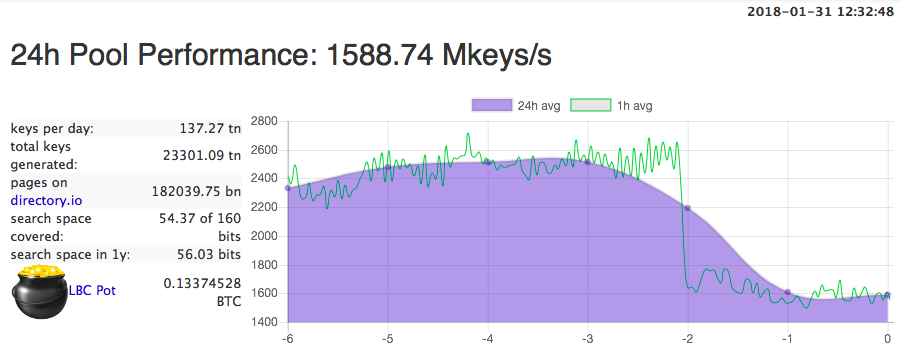
\includegraphics[width = .9\textwidth]{LBC.png}
				\caption{Bitcoin Full Node\supercite{TheLargeBitcoinCollider}}\label{LBC}
			\end{figure}

			如何建構一個亂數,在過往的亂數產生器往往會加入時間作為參數,但對於一個攻擊者而言,只需要去猜測在這段時間內目標者所有生成的可能性有極高的機率可猜出亂數。而亂數在密碼學中常會是一把私鑰的生成,在https協議中,服務器端與客戶端,建立一個加密連線的過程中也需要一個亂數去建立一個高安全性的加密通道-傳輸層安全性協定(Transport Layer Security,TLS)\supercite{dierks2008transport},在SSH協議中也採用了亂數。
	
			在過去的歷史事件中,發現Android手機版以及平板版的亂數產生器中存在著不隨機,於2013年8月比特幣開發者Mike Hearn提及“All private keys generated on Android phones/tablets are weak and some signatures have been observed to have colliding R values” \supercite{SomeSecureRandomThoughts},Bitcoin.org也發布了警告\supercite{AndroidSecurityVulnerability}簡要說明該事件的原因,以及表明影響到的Bitcoin Wallet 客戶端有Bitcoin Wallet、BitcoinSpinner、Mycelium Bitcoin Wallet、blockchain.info。這樣的錯誤源於Android本身支持的亂數產生器並不隨機,隨後Android解釋了亂數的問題並加以修正。在這Android手機亂數不夠亂的事件中,有自願者自發性地公布自己的損失狀態,總金額為55.82152538個比特幣\supercite{Badsignaturesleading},但因為比特幣屬於被動的性質,無人主動回報即不會加入統計中,所以總損失估計會超過55.82152538個比特幣。

			\subsubsection{Secp256k1}
			在密碼學中有分對稱式加密與非對稱式加密,對稱式加密又分為信息流加密與信息塊加密,信息流加密著名的是由美國密碼學家Ron Rivest教授設計,包括RC2(1987年)\supercite{OnthedesignandsecurityofRC2}、RC4(1987年)\supercite{Rc4}、RC5(1994年)\supercite{TheRC5encryptionalgorithm}、RC6(1998年)\supercite{TheRC6blockcipher.v1.1August201998};信息塊加密著名的有数据加密标准(Data Encryption Standard,DES,1975年)\supercite{Dataencryptionstandard}、三重数据加密算法(Triple Data Encryption Algorithm,Triple DES,1998年)\supercite{TrippleDataEncryptionAlgorithmModesofOperation}、高级加密标准(Advanced Encryption Standard,AES,1998年)\supercite{ThedesignofRijndael:AES-theadvancedencryptionstandard};非對稱式加密最廣為人知的有RSA(Rivest–Shamir–Adleman,1977年)\supercite{Cryptographiccommunicationssystemandmethod}、椭圆曲线密码学(Elliptic curve cryptography,ECC,1985年)\supercite{Ellipticcurvecryptosystems}。
			非對稱式加密與對稱式加密最大的不同在於,對稱式加密在加密解密的過程中只需要一把鑰匙,而非對稱式加密會生成兩把鑰匙分別為私鑰與公鑰,在算法的設計上一開始會以亂數產生一把私鑰,再經由非對稱式加密算法推導出公鑰,推導出的公鑰在非對稱式密碼學中並無直接的方法可以反推至私鑰,如此一來確立私鑰的安全性。非對稱式密碼的使用場景有兩種,第一種是希望收到加密信息的Alice,Alice會生成私鑰存儲在自己本地端的電腦中,並將推導出的公鑰公布在網路上,這時希望聯繫Alice的Bob在網路上取得公鑰後,Bob會以Alice的公鑰進行加密,之後將密文寄送給Alice,在傳遞信息的過程中,既使網路存在著監聽,也無法將信息順利解密,唯有Alice收到信息後使用Alice原本產生該公鑰的私鑰,才可以解出明文。第二種則應用在比特幣的交易之數字簽名以及交易驗證交易,比特幣地址的創建過程中會透過secp256k1生成私鑰公鑰對,在創建比特幣交易的過程中,使用該地址的私鑰對該地址未花费的输出(Unspent Transaction Output,UTXO)進行數字簽名,完成數字簽名後會與公鑰以及交易信息一起廣播到比特幣網路的交易緩池持當中,比特幣交易緩存池存在於所有比特幣全節點當中,主要存儲所有未被收入到比特幣區塊鏈內的所有交易,也就是零確認交易,等待礦工將該筆交易收入至比特幣區塊鏈當中。
			比特幣採用的secp256k1是屬於椭圆曲线密码学中的一個版本,不同的橢圓曲線版本的差異在於不同的初始參數,包括橢圓曲線方程$$y^2=x^3+ax+b$$、$p$=FFFFFFFFFFFFFFFFFFFFFFFFFFFFFFFFFFFFFFFFFFFFFFFFFFFFFFFEFFFFFC2F為巨大的質數、G點被称为⽣成点的常数点亦稱為基點。至於為什麼選擇ECC而非RSA的主要原因,其一在於ECC在生成密鑰對所需的時間更佳快速,圖\ref{ECCtime}為Nicholas Jansma於2004年針對ECC與RSA的密鑰對生成時間與數字簽名所需時間的論文\supercite{Performancecomparisonofellipticcurveandrsadigitalsignatures}顯示,當ECC產生571 bits的密鑰長度,RSA要達到相同的安全性需要生成15360 bits,這也導致生成時間產生高達471倍之差距。
			
			\begin{figure}[h]
				\centering
				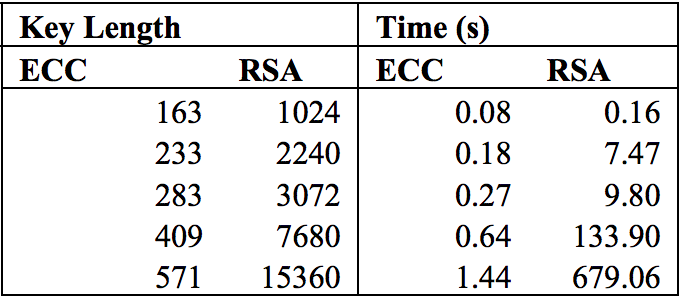
\includegraphics[width = .5\textwidth]{ECCtime.png}
				\caption{ECC與RSA的密鑰對生成時間\supercite{Performancecomparisonofellipticcurveandrsadigitalsignatures}}\label{ECCtime}
			\end{figure}

			除了在密鑰對生成時間ECC有著比RSA更高效的算法外,在安全性上ECC可以更短的密鑰長度達到與RSA相同的安全強度,L Ducas針對ECC、RSA、BLISS做出了深度的安全性探討\supercite{LatticesignaturesandbimodalGaussians},圖\ref{LatticesignaturesandbimodalGaussians}同樣達到80 bits的安全性級數,RSA 1024需要1024 bits,ECDSA 160僅需要160 bits,該篇論文除了探討RSA與ECDSA之外,更大的部分在闡述量子計算機對於既有的傳統密碼帶來的抨擊,有機會快速窮舉$2^{256}$的比特幣私鑰,在未來量子計算機的蓬勃發展擁有2000 qbits運算能力,量子計算機可以快速窮舉破解所有的比特幣私鑰。因此發展針對量子計算機設計的數字簽名算法成為密碼學上嶄新的議題,而BLISS則為針對量子計算機所設計的抗量子計算的簽名算法。

			\begin{figure}[h]
				\centering
				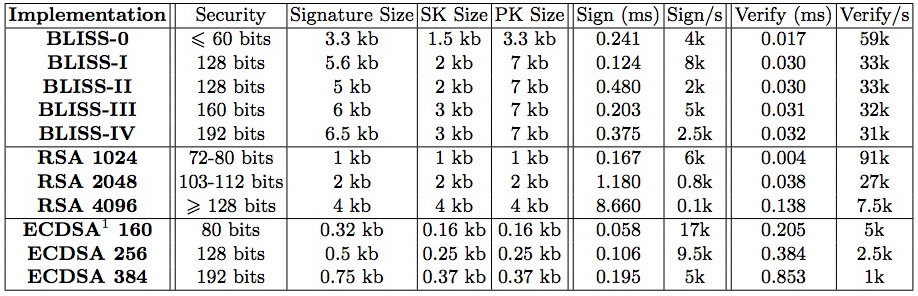
\includegraphics[width = 1\textwidth]{LatticesignaturesandbimodalGaussians.png}
				\caption{算法BLISS、RSA、ECDSA安全級數比較\supercite{LatticesignaturesandbimodalGaussians}}\label{LatticesignaturesandbimodalGaussians}
			\end{figure}

			\subsubsection{SHA-256}
			哈希下數在比特幣系統中扮演著相當多的角色,包括比特幣地址生成、比特幣交易哈希指針、比特幣區塊哈希指針、比特幣挖礦算法工作量證明。哈希算法有幾大特色,分別為
			\subsubsection{RIPEMD-160}
			\subsubsection{Base58}

		\subsection{比特幣地址生成過程}

		\begin{figure}[h]
				\centering
				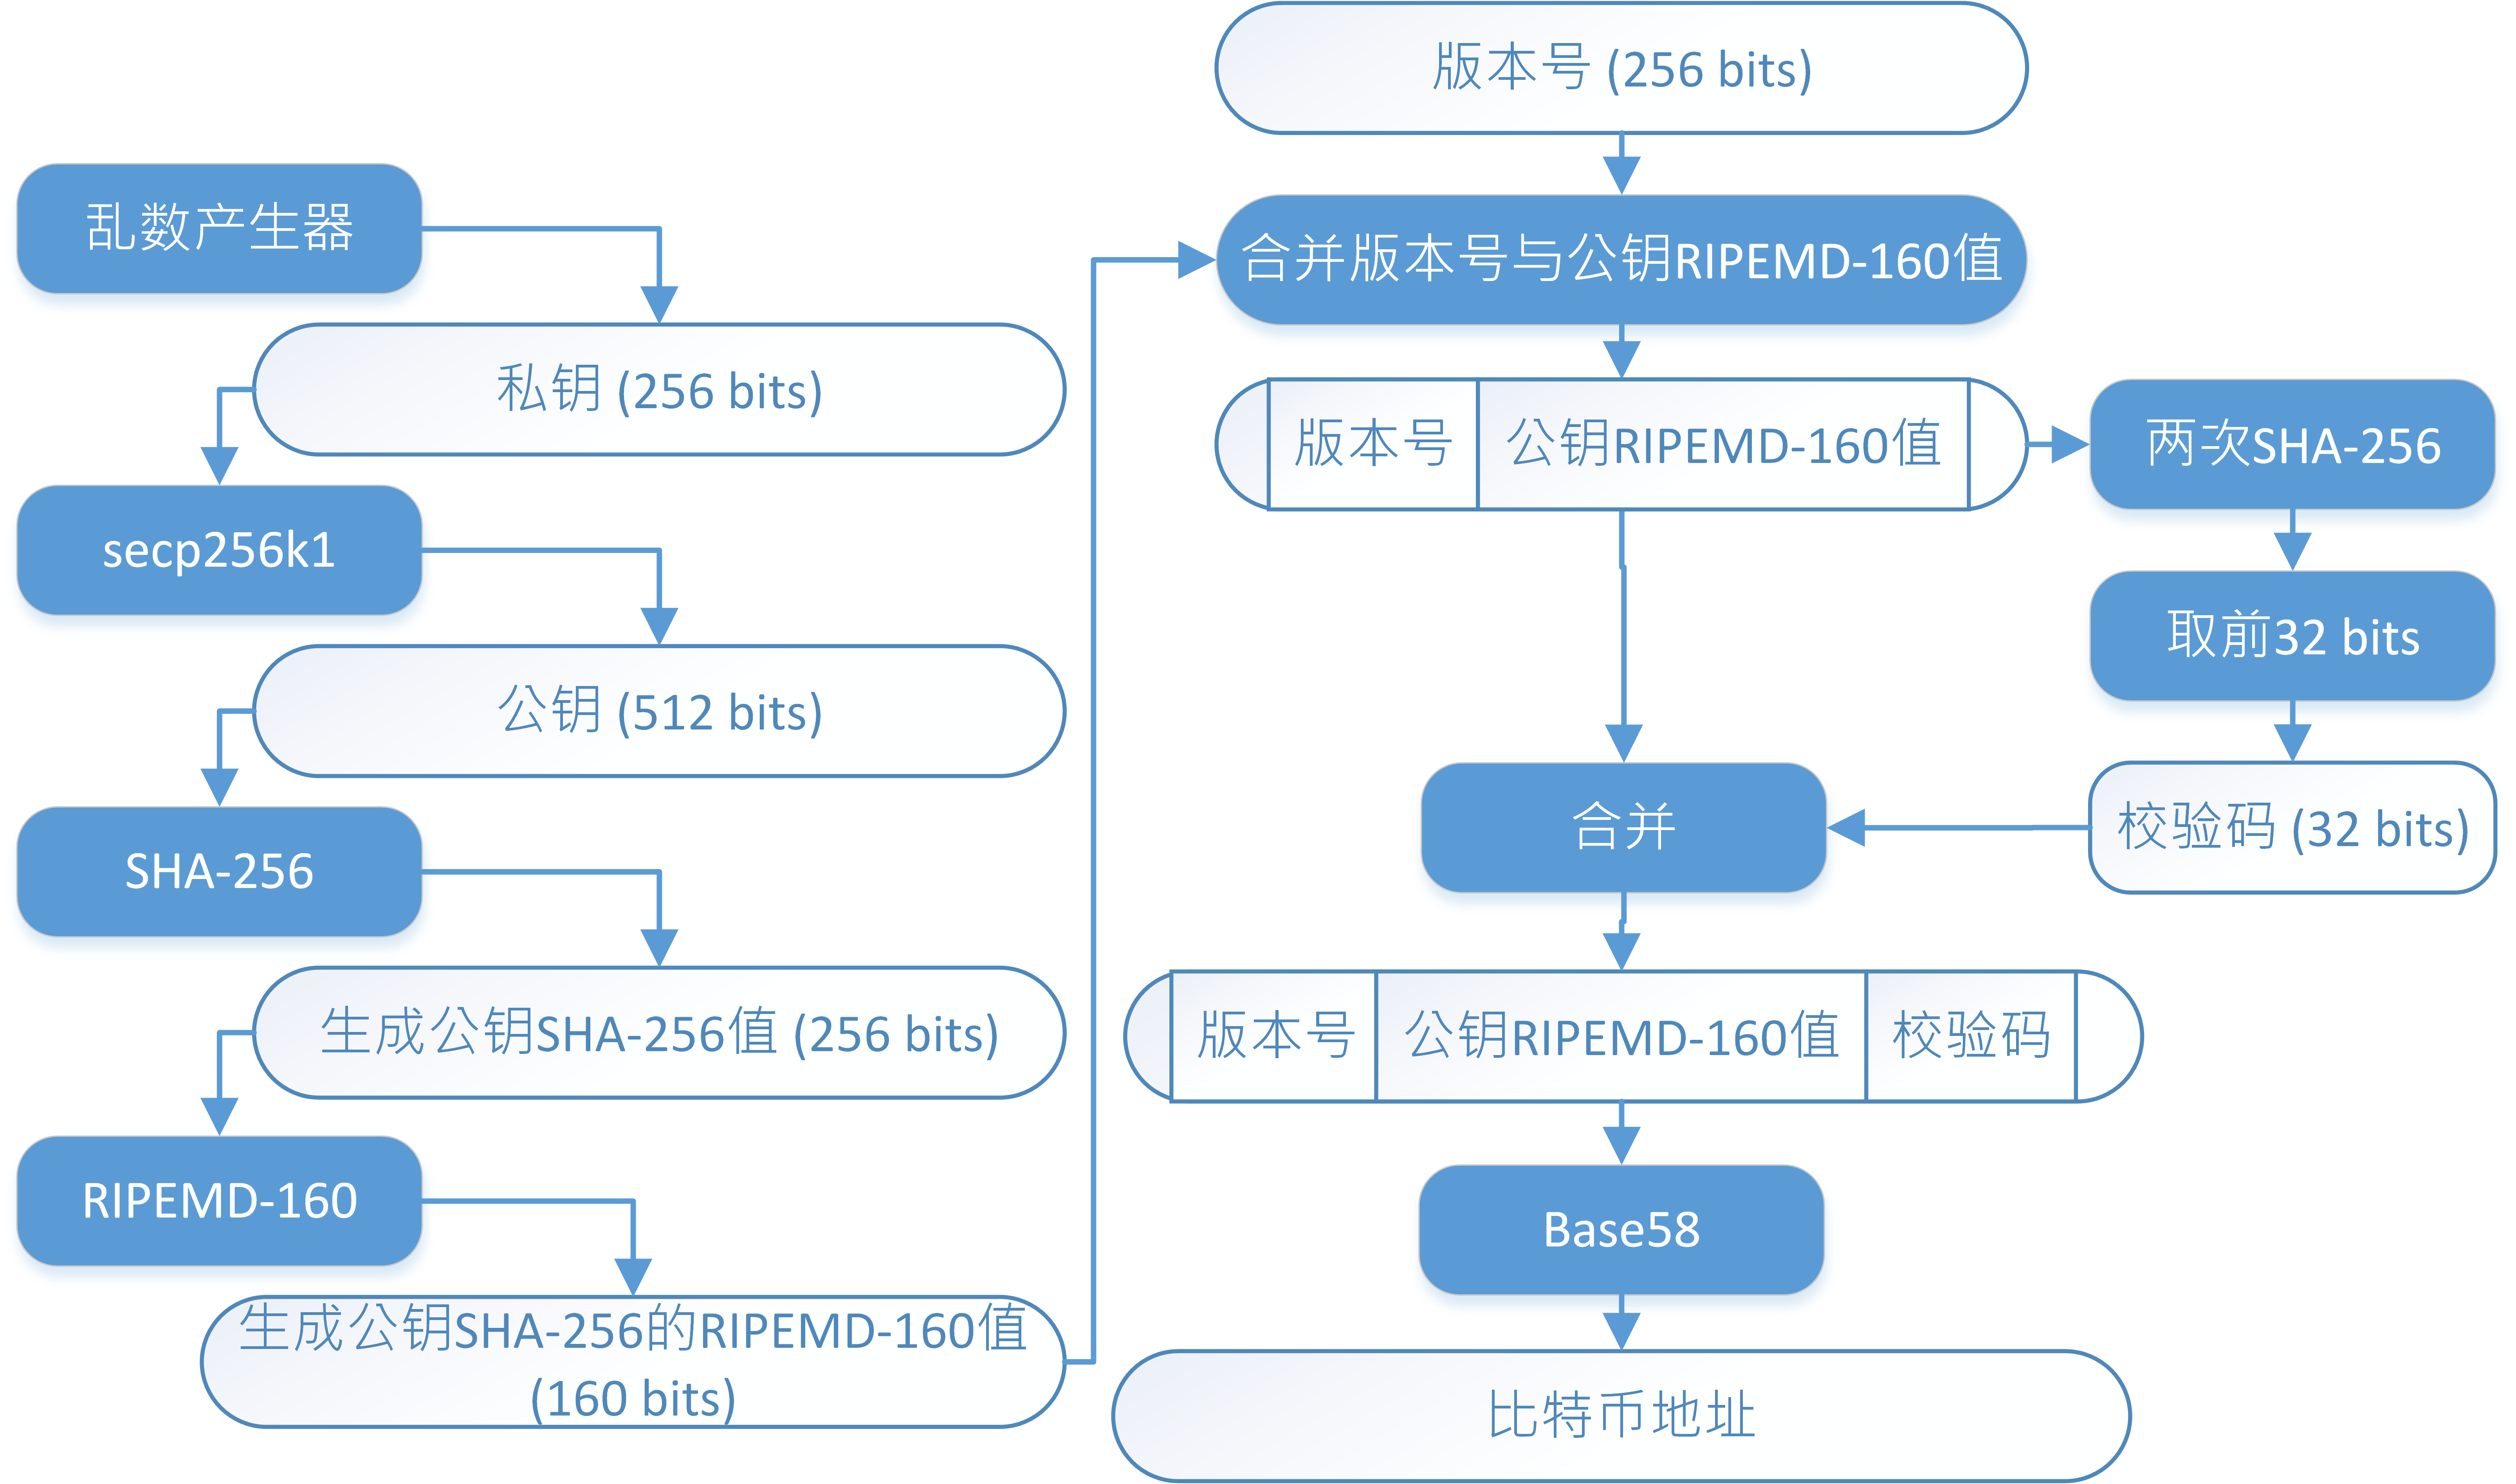
\includegraphics[width = .9\textwidth]{address.png}
				\caption{比特幣地址生成過程}\label{address}
		\end{figure}

		\begin{enumerate}
			\item 生成私鑰:使用亂數產生器產生一個長度在256 bits以內的隨機數,而此隨機數即成為該地址的私鑰,在比特幣系統中,可以利用私鑰(Private Key)簽署花費該地址當中的比特幣。
			\item 生成公鑰:該演算法為一個以橢圓曲線演算法為基礎的一個標準,而不同標準的差異在於初始化的參數,這些參數的訂定皆經過嚴謹的考核及實驗測試。在比特幣系統中該算法扮演著私鑰轉換為公鑰的角色。這使得比特幣交易使用私鑰進行簽署之後,還可以使用公鑰校驗該筆交易的正確性。
			\item 生成公鑰SHA-256:一種哈希函數,哈希函數的特性有許多,包括雪崩效應、不可預測、不可逆、校驗檔案是否完整。在此步驟中是將公鑰帶入SHA-256 函數中,產出長度為256 bits的哈希值。
			\item 生成公鑰SHA-256的RIPEMD-160:亦為哈希函數的一種,特色符合哈希函數的特性,與SHA-256不同的是RIPEMD-160產出的長度為160 bits。
			\item 取得版本號:比特幣在一開始設計的過程中,便定義了不同的地址樣式及功能,在第五個步驟中會加入版本號加以區分不同的地址。
			\item 校驗碼生成:校驗碼為比特幣地址生成過程中重要的一環,可在支付比特幣的過程中降低因為手誤而將比特幣轉入到不存在(不符合比特幣地址生成規則)地址的可能性。對公鑰SHA-256的RIPEMD-160再做兩次SHA-256,取該哈希值前32 bits的值作為校驗碼。
			\item 版本號、公鑰SHA-256的RIPEMD-160和校驗碼合併:版本號、第四個步驟的產生之公鑰RIPEMD-160及第五個步驟產生之校驗碼合併。
			\item 合併的結果以Base58編碼:將第六步驟組進行合併組合的結果,利用Base58進行編碼,Base58修改自Base64,其與Base64最大不同之處在於移除了"0"、"O"、"I"、"l"、"+"、"/"的字符,可以降低人工判讀在地址的錯誤率。
		\end{enumerate}

		\subsection{多重簽名(Multi-Signature)}
		% 	\subsubsection{多重簽名地址}
		 	\subsubsection{Green Address}
		 	雙重支付問題存在於比特幣交易在未被區塊鏈確認收入到區塊鏈之前,都有機會受到惡意的攻擊者雙重支付(Double-spending)\supercite{Informationpropagationinthebitcoinnetwork}同一筆款項。現今的比特幣區塊產出速度為十分鐘一塊,即便附上足夠的手續費也須等待將近十分鐘的時間,倘若是在手續費不足的情況下,該筆比特幣交易甚至會在比特幣交易緩存池中滯留一週的時間。在手續費足夠的情況下,十分鐘的確認時間會對實體店面的小額交易處理非常的不友善,為了在既有的比特幣區塊鏈的框架底下能夠提升交易速度,因此Green Address技術致力於在一開始創建交易的同時管控雙重支付交易的發生,他們採用了2-of-2多重簽章,也就是創建一個特殊的比特幣地址,這個比特幣地址的持有人有兩個代表人,分別為使用者與Green Address機構節點,這筆交易的建立必須要雙方同時簽署交易才被允許廣播至比特幣網路中。若是遇到交易塞車,且節點緩存池空間不足的問題時,比特幣節點會優先遺棄手續費最低的交易,視同此機交易不曾存在過,故若真的遇到交易被遺棄的情況,Green Address機構節點也會透內部的數據庫紀錄再次廣播此筆交易,並確保此筆交易可以被收入至區塊內。Green Address機構節點也就成為了交易創建的把關者,過濾所有的雙重支付攻擊的發生,也避免交易因為比特幣網路塞車而交易被礦工遺棄的情形。
		 	在這樣的機制下,只要是用Green Address錢包交易即可確認雙重支付攻擊是不會發生的,對商家或是收款人而言,可以得到在即時交易中不被雙重支付攻擊的保障,提升在未進入區塊鏈的交易可確定性,進而創造出即時交易的可行性。

		 	\paragraph{Green Address錢包生成過程}
		 	此節將詳細闡述Green Address錢包生成過程的重要步驟,如圖\ref{gabuild}所示。
		 	\begin{figure}[h]
				\centering
				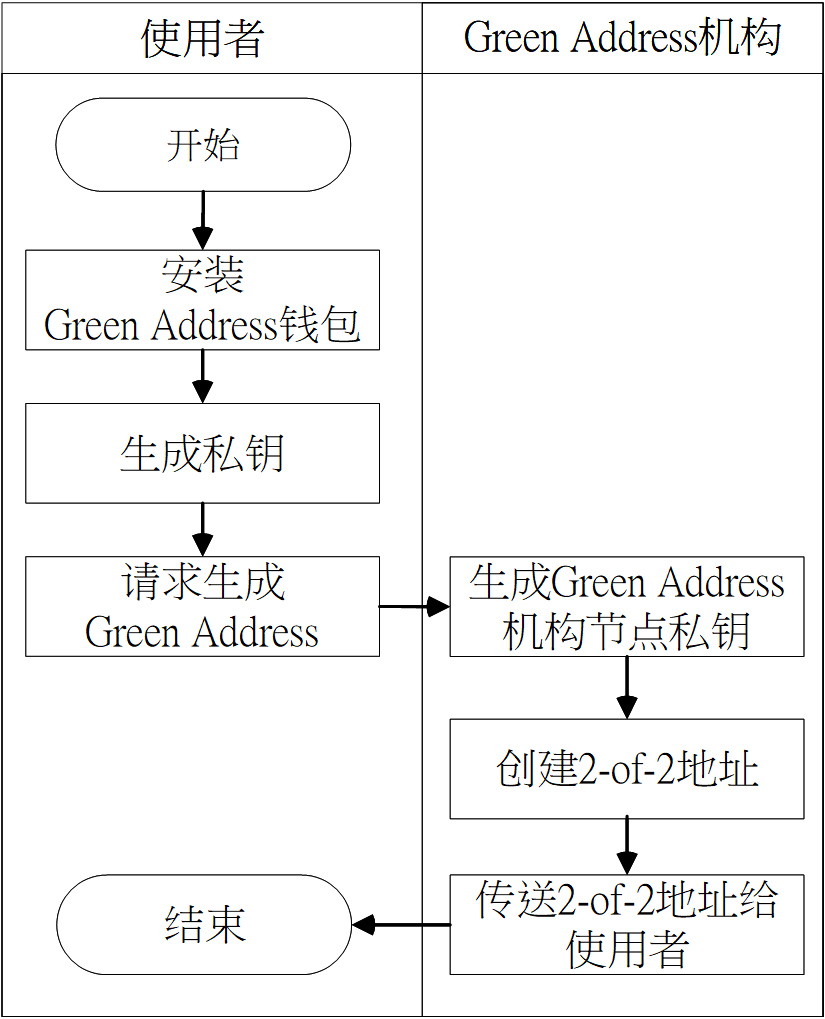
\includegraphics[width = .5\textwidth]{gabuild.png}
				\caption{Green Address錢包生成過程}\label{gabuild}
			\end{figure}

		 	\begin{enumerate}
		 		\item 使用者安裝Green Address比特幣錢包,並向Green Address機構節點請求創建2-of-2多重簽章比特幣地址。
		 		\item 使用者與Green Address機構節點分別生成兩把私鑰,共同創建Green Address比特幣地址。
		 		\item 當交易發起時,使用者使用自己的私鑰簽署該筆交易。
		 		\item 將該筆交易傳送到Green Address機構節點。
		 		\item Green Address機構節點收到後,檢查該筆交易是否存在雙重支付攻擊。
		 		\item 確認無攻擊跡象後便廣播至比特幣網路中。
		 	\end{enumerate}

		 	\paragraph{Green Address交易發起流程}
		 	說明完Green Address地址是如何創建之後,該節將詳細說明如何運用多重簽章地址發起交易至比特幣網路中,如圖\ref{gatx}所示。

		 	\begin{figure}[h]
				\centering
				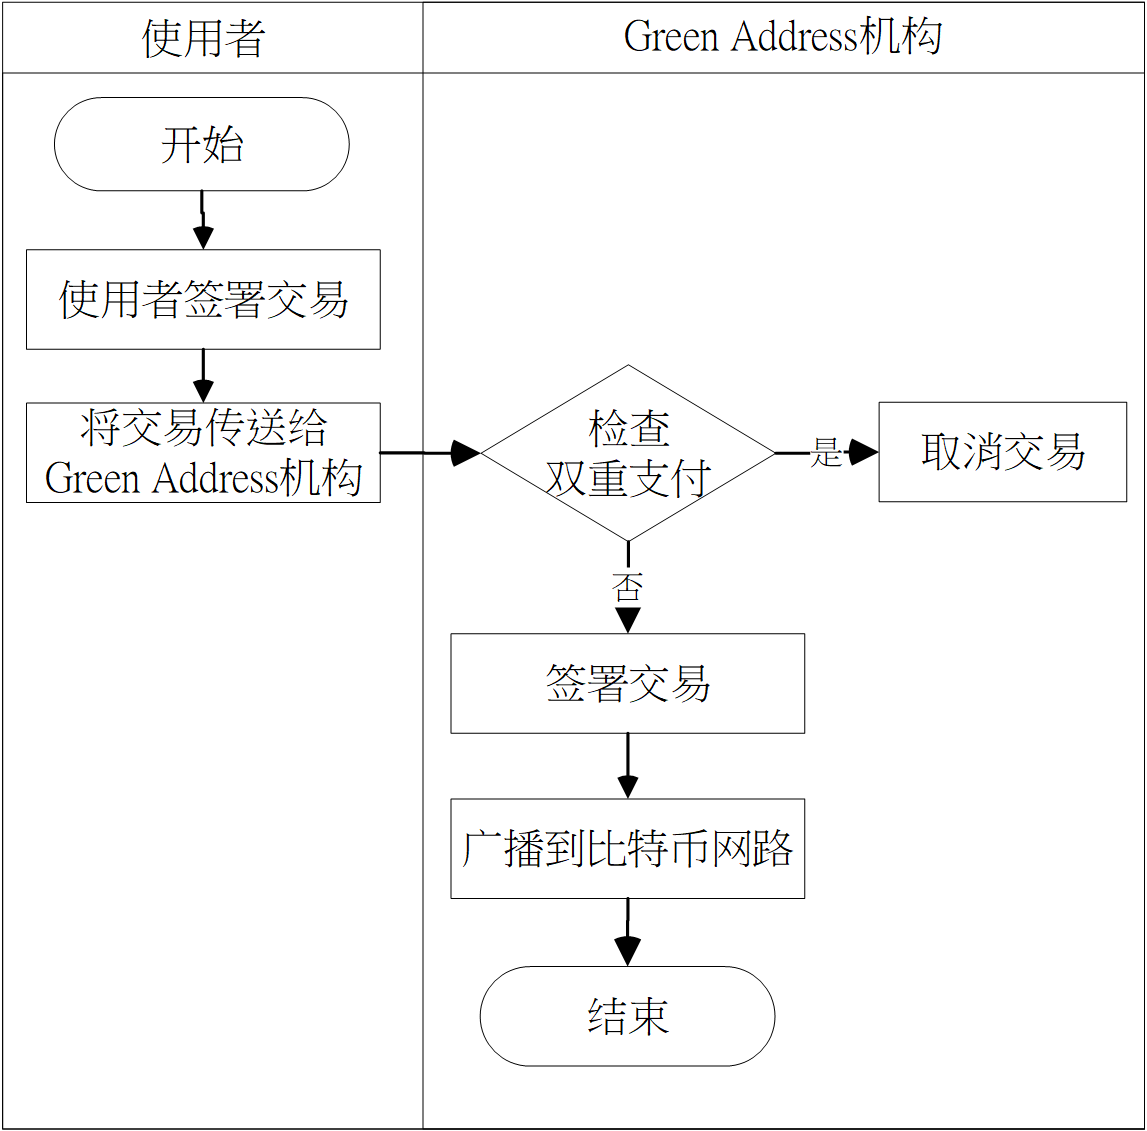
\includegraphics[width = .7\textwidth]{gatx.png}
				\caption{Green Address交易發起流程}\label{gatx}
			\end{figure}

			\begin{enumerate}
				\item 使用者使用原本創建Green Address的私鑰,並完成簽署交易。
				\item 因為是多重簽章地址,所以該交易需傳送至Green Address機構節點。
				\item Green Address機構節點收到交易信息後檢查該交易的發起地址是否存在雙重支付,倘若有雙重支付則遺棄;若無雙重支付則往下一個步驟。
				\item Green Address機構以Green Address的私鑰簽署該筆交易。
				\item 將該筆交易封包廣播至比特幣網路。
			\end{enumerate}

	\section{區塊鏈(Blockchain)}
	%區塊頭所有的結構
	自2009年以來,密碼貨幣比特幣的誕生引發了新的貨幣革命浪潮,基於密碼學,點對點網絡,共識算法和區塊鏈技術,它們被結合成比特幣等密碼貨幣。到目前為止,它在九年內發生大量的襲擊和欺詐事件後仍然在積極努力。 比特幣一直是互聯網上最具代表性的密碼貨幣。比特幣是區塊鏈技術最重要的應用之一。我們將描述區塊鏈技術的一些細節。

		%%%%%%\subsection{本區塊大小的值 }
		\subsection{區塊頭(Block Header)}

		\begin{figure}[h]
			\centering
			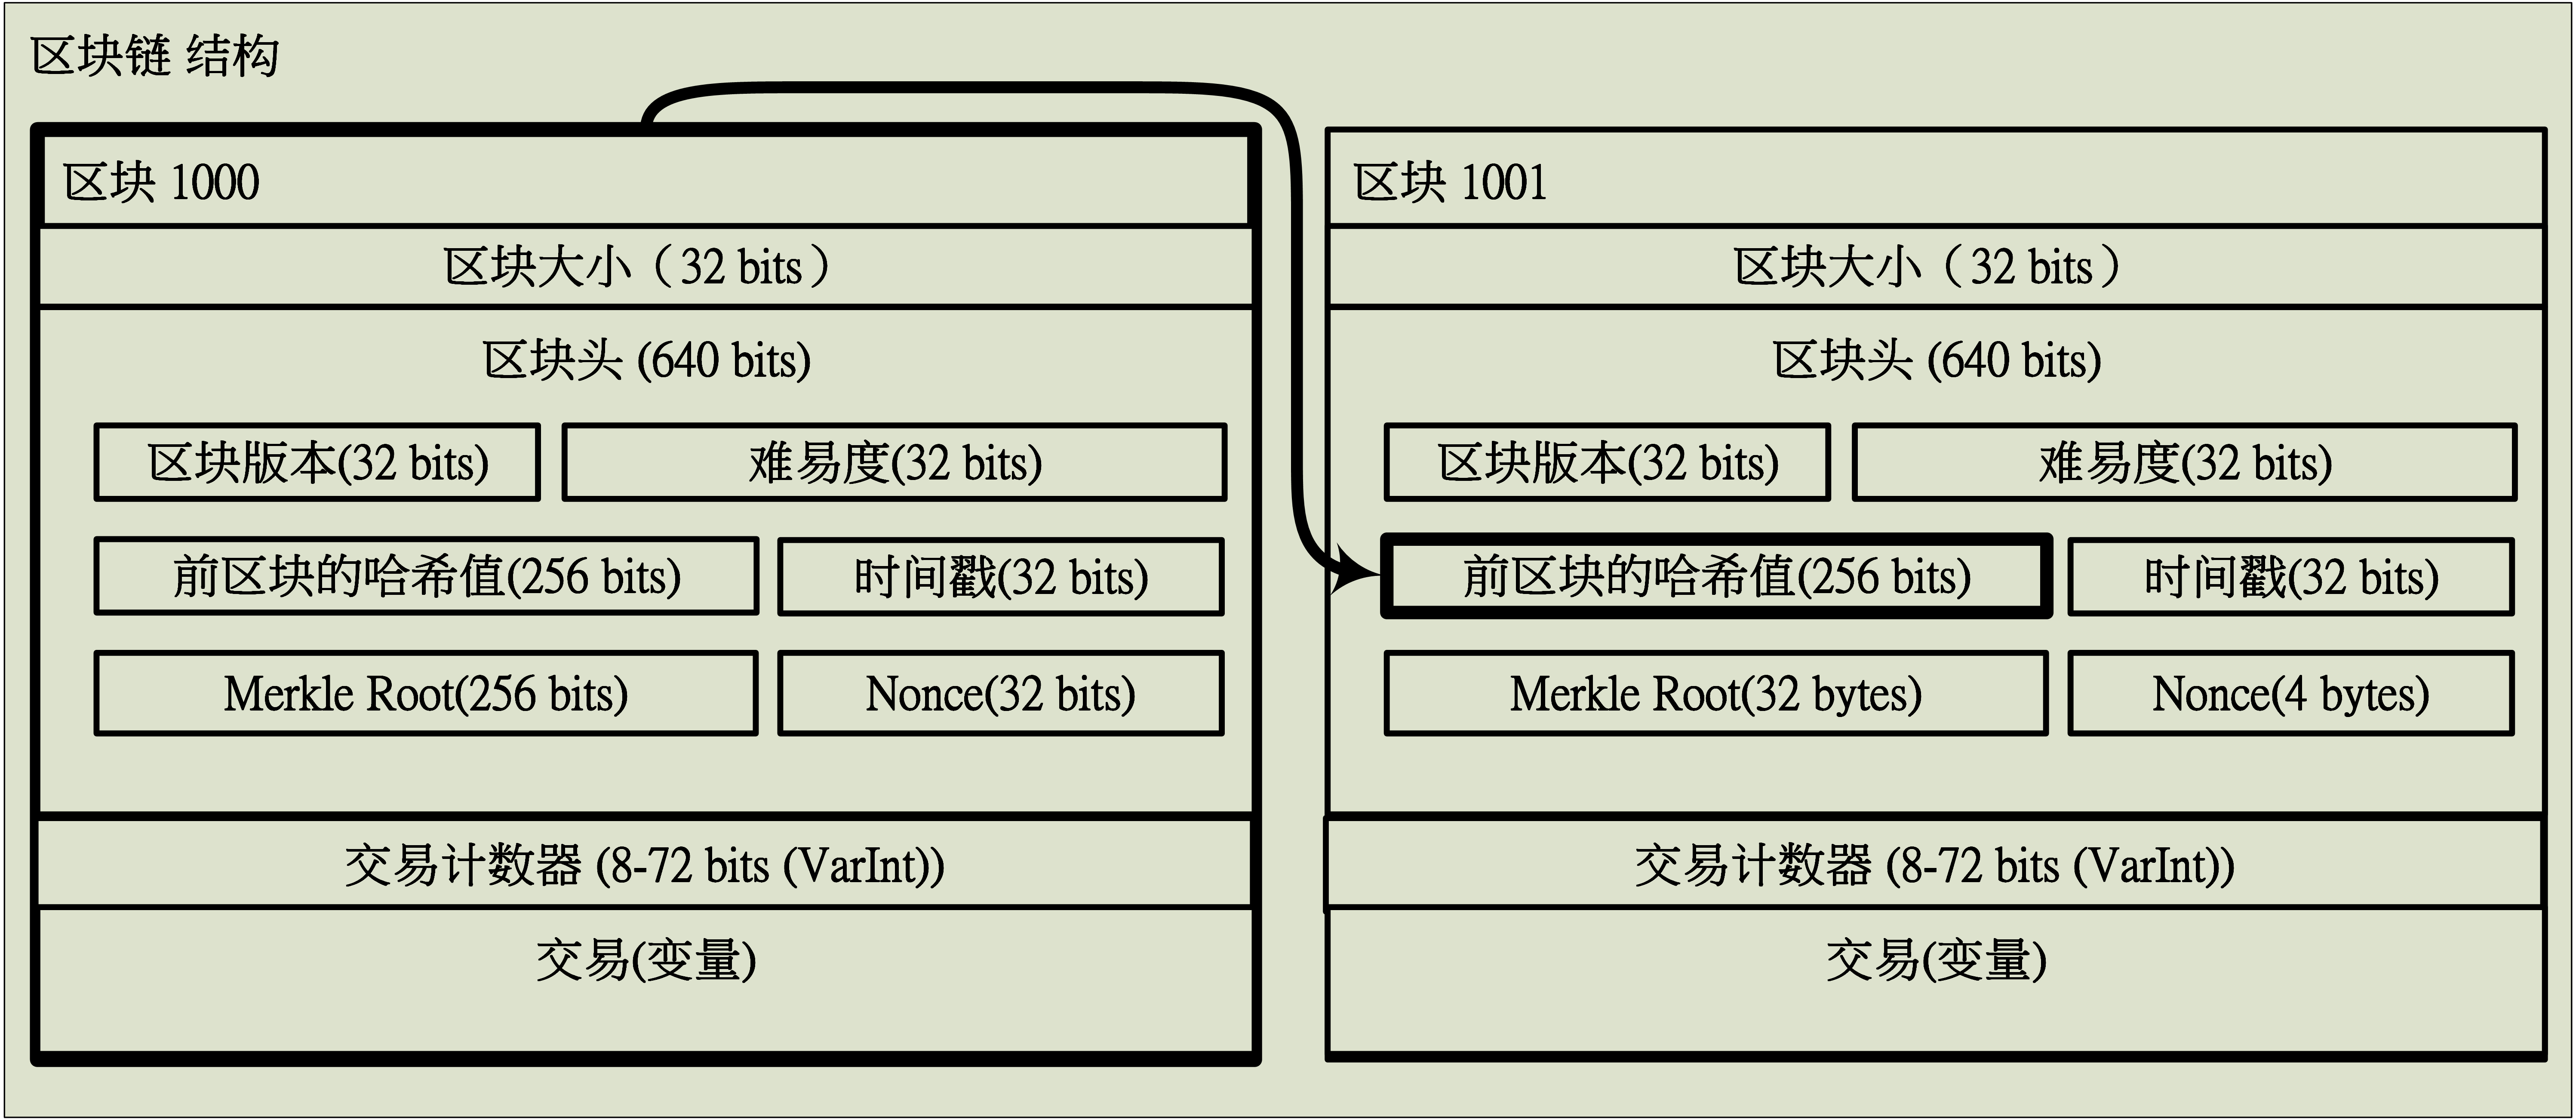
\includegraphics[width = 1\textwidth]{blockchain.png}
			\caption{比特幣區塊鏈結構}\label{blockchain}
		\end{figure}

			\paragraph{區塊版本(32 bits)}該欄位存儲比特幣區塊鏈中的區塊版本。
			\paragraph{前區塊的哈希值(256 bits)}記錄前一個塊的哈希值。 根據當前區塊的前一個區塊哈希值進而形成哈希指針,所有塊可以因為哈希指針連接在一起形成比特幣區塊鏈,不僅可以在區塊與區塊間建立虛擬鏈接,還可以使得區塊更難以被篡改。為新區塊不斷疊加在舊的區塊上,舊區塊的哈希值將繼續傳遞到最新的區塊。若區塊上面堆疊更多的區塊,促使的哈希值間接引用越多次,因此較早創建的區塊更難以修改。
			\paragraph{Merkle Root(256 bits)}Merkle Root的生成方法是將當前區塊的所有交易為n個進行排序後,此時的交易為n個樹葉,將每個樹葉進行一次SHA-256哈希算法取得哈希值得到$n$個哈希值,再將哈希值兩兩配對合併進行哈希,得到$n*2^{-1}$個哈希值後,在$k$輪後會使得$n*2^{-k}=1$時,合併到只剩下一個哈希值,最後一個哈希值則為Merkle Root,如圖所示\ref{MerkleRoot},在區塊鏈中的Merkle Root可用於快速檢查當前區塊中所有存儲交易的正確性。

			\begin{figure}[h]
				\centering
				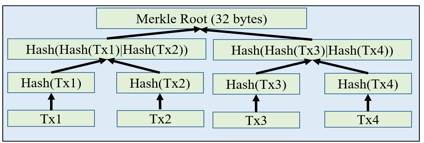
\includegraphics[width = 0.7\textwidth]{MerkleRoot.png}
				\caption{Merkle Tree}\label{MerkleRoot}
			\end{figure}

			\paragraph{難易度(32 bits)}在比特幣網路中難易度參數平均每十五天會有所變動,用以調控比特幣區塊的產出頻率,在過去的密碼貨幣的設計中,有著因為沒有動態修改區塊難度,而導致區塊鏈生成速度太快,甚至導致區塊鏈系統崩潰。
			\paragraph{時間戳記(32 bits)}以年、月、日、小時和秒的格式記錄區塊生成時間。
			\paragraph{Nonce(32 bits)}Nonce記錄著礦工在進行挖礦時,必須要不斷的嘗試Nonce參數,直到符合難易度參數,才可以創建一個全新的比特幣區塊。該值為32 bits ,意為著礦工嘗試的組態空間為$2^{32}$個可能性。

	%區塊內容 交易手續費攻擊
		%\subsection{Block Data}
		%	\subsubsection{交易計數器 (4-36 bits)}
		%	\subsubsection{交易信息}

	%\section{工作量證明(Proof of Work)}
	\section{點對點網路(Peer to peer network)}

	去中心化的密碼貨幣系統帶給社會帶給傳統的中心化的金融體系以及政府帶來了很重大的衝擊,中本聰建構了一個不需要中央銀行發行貨幣的貨幣系統,在比特幣的貨幣發行上全靠區塊鏈既定的算法。除了貨幣發行,也將交易紀錄的帳本已明文的方式儲存在去中心化的區塊鏈中,以比特幣為例,現今的完整的比特幣區塊鏈帳本已經高達180GB,這樣保存完整交易資料的計算機稱之為全節點,在比特幣去中心化的網路中,如圖\ref{bitcoinfullnode}所示,截至2018年1月25比特幣網路中全節點數量為10552個\supercite{bitcoinfullnode},全節點的數量決定了比特幣帳本的可靠度,倘若有著更多的全節點,會使得比特幣網路堅不可摧,更難去修改歷史發生過的交易數據。

	\begin{figure}
		\centering
		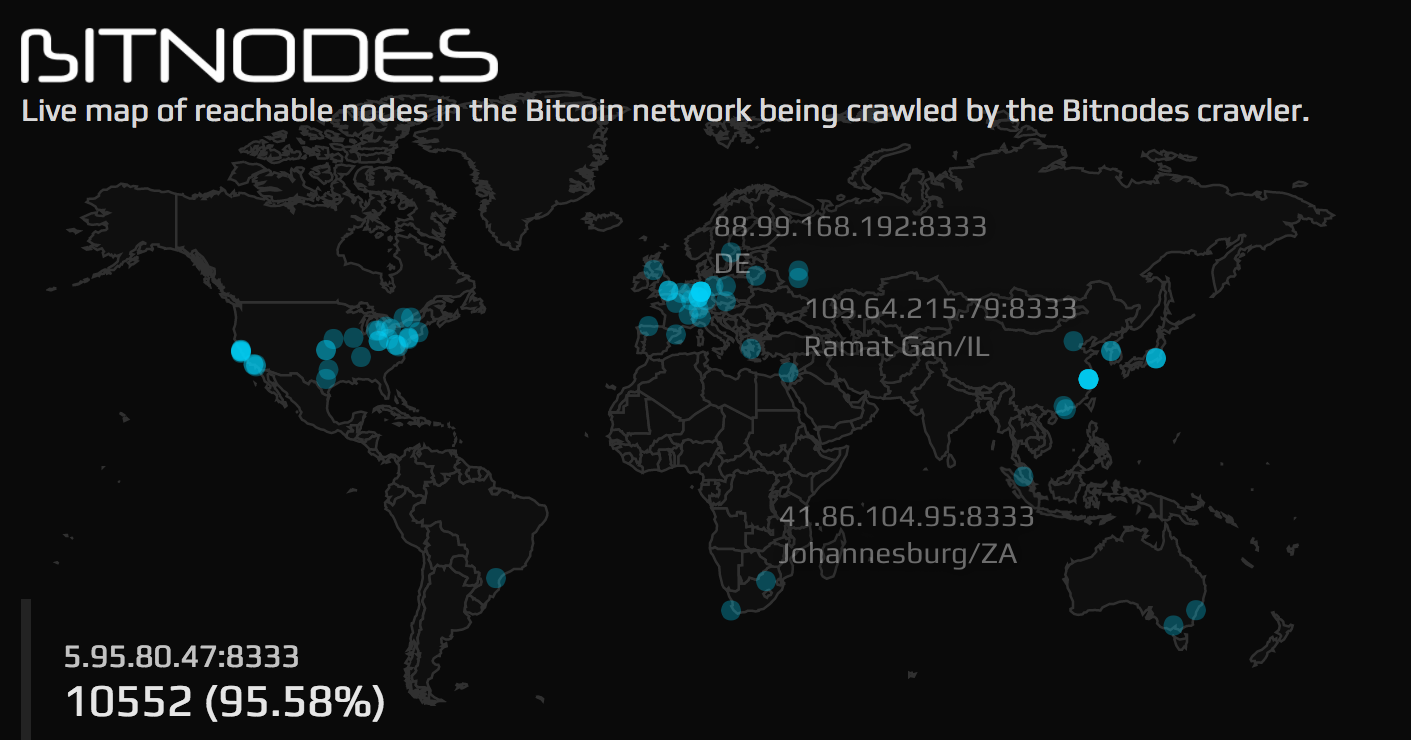
\includegraphics[width = .9\textwidth]{bitcoinfullnode.png}
		\caption{Bitcoin Full Node\supercite{bitcoinfullnode}}\label{bitcoinfullnode}
	\end{figure}

	% \section{山寨幣(Altcoin)簡介}

	% 	\subsection{萊特幣(Litecoin)}

	% 	\subsection{狗幣(Dogecoin)}

	% 	\subsection{域名幣(Namecoin)}

	% 	\subsection{以太坊(Etherum)}